\PassOptionsToPackage{hyperfootnotes=false}{hyperref}
\documentclass{beamer}
\usefonttheme{professionalfonts}
%\usetheme{Rochester}
%\usetheme{AnnArbor}
\usetheme{Szeged}
\useoutertheme{infolines}
\usecolortheme{dolphin}
\usepackage{graphicx}
% \usepackage[english]{babel}
\usepackage{multicol}
\usepackage{color}
\usepackage{xcolor}



%\definecolor{carmine}{rgb}{0.59, 0.0, 0.09}
\usepackage{amsmath} 

\usepackage{graphicx}
\usepackage{tikz}
\usetikzlibrary{shapes.callouts}
\usepackage{multirow}

\usepackage[utf8]{inputenc}

\usepackage{enumerate}
\usepackage[shortlabels]{enumitem}
\usepackage{amsmath,amsthm,amssymb,amsfonts,mathrsfs,latexsym,stmaryrd}
\usepackage{tcolorbox}

\usepackage{color} 
\usepackage{amssymb, amsmath, amsbsy}
\usepackage{adjustbox,lipsum}
\usepackage{placeins}

\usepackage{textpos}
\usepackage{wrapfig}
\usepackage[spanish, es-tabla]{babel}

\usepackage{caption}
\setlength{\parindent}{0pt}

\usepackage{url}
\usepackage{float}
\usepackage{tikz}
\usetikzlibrary{patterns}


\title[ICS-162]{Econometría ICS-294\\ \small{Clase 11: Inferencia sobre un conjunto de parámetros}}

\author{Francisco Alfaro Medina}
\institute[USM]
{Universidad Técnica Federico Santa María\\ % Your institution for the title page
	\medskip
	\textit{} % Your email address
	
}
\logo{

\includegraphics[width=1cm]{Logo.png}
}
\date{}
\newcommand\Fontvi{\fontsize{9}{7.2}\selectfont}
\begin{document}
	
\begin{frame}
	\titlepage % Print the title page as the first slide


\end{frame}
%%%%%%%%%%%%%%%%%%%%%%%%%%%%%%%%%%%%%%%%%%%%%%%%%%%%%%%%%%%%%%%%%%%%%%%%%%%

\begin{frame}[shrink=10]{Test de hipótesis sobre un conjunto de parámetros}
    \begin{itemize}
        \item A menudo estamos interesados en testear hipótesis para varios parámetros a la vez.
        
        \item Por ejemplo si dos coeficientes son 0 al mismo tiempo.
        \item En ese caso, las hipótesis se verían de la siguiente forma:
        \begin{align*}
            H_0 & : \beta_{\text{1}} = \beta_{\text{2}} = 0 \\
            H_1 & :  \text{Al menos uno }\neq 0
        \end{align*}
        \item Cuando se rechaza la hipótesis nula se dice que $x_1$ y $x_2$ son conjuntamente significativas al correspondiente nivel de significancia.
        \item Noten que en este caso, el test NO dice cuál de las variables tiene un efecto en \( y \). Puede ser una sola, varias o todas.
        \item Para esto vamos a usar un estadístico F.
    \end{itemize}
\end{frame}

\begin{frame}{Repaso relevante para esta clase}
    Partiendo de \( y = \beta_0 + \beta_1 x_1 + \beta_2 x_2 + \ldots + \beta_k x_k + u \), calculo por MCO y obtengo la predicción: \( \hat{y} \). Definiciones:
    \begin{center}
        \( SST : \sum_i (y_i - \bar{y})^2 \) $\rightarrow$ variabilidad de \( y \)\\
        \( SSE : \sum_i (\hat{y}_i - \bar{y})^2 \) $\rightarrow$ lo explicado por mi modelo\\
        \( SSR : \sum_i \hat{u}_i^2 \) $\rightarrow$ lo que mi modelo no explica/se equivoca\\
        \( SST : SSE + SSR \) $\rightarrow$ lo que explico + lo que no explico con mi modelo\\
        \( R^2 : 1 - \frac{SSR}{SST} \) $\rightarrow$   fracción de la  variabilidad de \( y \) que es explicada por mi modelo
    \end{center}
\end{frame}

\begin{frame}{Repaso: Si agrego variables relevantes, cae mi SSR}

    Supongan que parto estimando $y = \beta_0 + \beta_1 x_1 + u$.
    \begin{itemize}
        \item SST = SSE + SSR
        \item SST = lo que explico + lo que no explico con el modelo
        \item $R^2 = 1 - \frac{SSR}{SST}$ \\ 
        \quad \textit{el \% de la variabilidad de y que es explicada por mi modelo}
    \end{itemize}

    ¿Qué pasa si agrego a mi modelo una variable $x_2$ relevante para explicar $y$?
\end{frame}

\begin{frame}{Repaso: Si agrego variables relevantes, cae mi SSR}

    Supongan que parto estimando $y = \beta_0 + \beta_1 x_1 + u$.
    \begin{itemize}
        \item SST = SSE + SSR
        \item SST = lo que explico + lo que no explico con el modelo
        \item $R^2 = 1 - \frac{SSR}{SST}$ \\ 
        \quad \textit{el \% de la variabilidad de y que es explicada por mi modelo}
    \end{itemize}

    ¿Qué pasa si agrego a mi modelo una variable $x_2$ relevante para explicar $y$? Cae mi $SSR$ y aumenta mi $R^2$.

\[ \text{SST} = \textcolor{red}{\uparrow \text{SSE}} + \textcolor{red}{\downarrow \text{SSR}} \]
\vspace{0.25cm}
\[ \textcolor{red}{\uparrow} R^2 = 1 - \frac{\textcolor{red}{\downarrow \text{SSR}}}{\text{SST}} \]

\end{frame}



\begin{frame}[t]{Test de hipótesis y modelo restringido}
    \begin{itemize}
    \item Entonces, una buena forma de testear si variables son irrelevantes para
    explicar la variable $y$ (tienen $\beta's = 0$) es:
    
    \item Mirar las diferencias entre el SSR de un modelo que las incluye (modelo
        unrestricted: $SSR_{ur}$) y el SSR de un modelo que no las incluye (modelo
        restricted: $SSR_{r}$).
        \item Cuanto más grande sea la diferencia $SSR_{r} - SSR_{ur}$ más seguros estaremos de
        que las variables en cuestión son relevantes para explicar $y$.
        \item ¿Cuál es el signo de esta diferencia $SSR_{r} - SSR_{ur}$?
        \pause
        \item \(SSR_{r} - SSR_{ur} \geq 0\)
    \end{itemize}
\end{frame}

\begin{frame}[t]{Test: Definiciones}
\begin{itemize}
    \item Sea el modelo: \( y = \beta_0 + \beta_1 x_1 + \beta_2 x_2 + \beta_3 x_3 + u \)
    \item Nos interesa testear si \( x_2 \) o \( x_3 \) o ambas son relevantes para el modelo.
    Es decir: \( H_0: \beta_2 = \beta_3 = 0 \), \( H_1: \text{Al menos uno }\neq 0\)
\end{itemize}
\end{frame}

\begin{frame}[t]{Test: Definiciones}
\begin{itemize}
    \item Sea el modelo: \( y = \beta_0 + \beta_1 x_1 + \beta_2 x_2 + \beta_3 x_3 + u \)
    \item Nos interesa testear si \( x_2 \) o \( x_3 \) o ambas son relevantes para el modelo.
    Es decir: \( H_0: \beta_2 = \beta_3 = 0 \), \( H_1: \beta_2 \neq 0 \) o \( \beta_3 \neq 0 \).

    \textbf{Modelo no restringido (UR)}: se incluyen todas las variables.
    \begin{itemize}
        \item Estimando el modelo no restringido por MCO, \( y = \beta_0 + \beta_1 x_1 + \beta_2 x_2 + \beta_3 x_3 + u \) 
        \(\rightarrow\) \textcolor{red}{obtenemos
\( SSR_{ur} \)}
    \end{itemize}
    
    \textbf{Modelo Restringido (R)}: se asume \( H_0 \) verdadera y se estima el modelo:
    \begin{itemize}
        \item \( y = \beta_0 + \beta_1 x_1 + u \)
        \(\rightarrow\) \textcolor{red}{obtenemos \( SSR_r \)}
    \end{itemize}
    
    \item Rechazamos \( H_0 \) a medida que \( SSR_r - SSR_{ur} \) sea mayor. Si se cumpliera \( H_0 \), es decir las variables \( x_2 \) y \( x_3 \) fueran totalmente irrelevantes, esa diferencia sería cercana a 0.
\end{itemize}
\end{frame}

\begin{frame}[t]{Test de hipótesis y modelo restringido}
    \begin{itemize}
        \item Podemos pensar el test de hipótesis como la comparación entre el modelo
        original y el modelo restringido (cuando se cumple la $H_0$).
        \item Entonces, se puede demostrar que:
    \end{itemize}
    \vspace{0.5cm}
    \[
    F = \frac{SSR_{r} - SSR_{ur}}{SSR_{ur}} \cdot \frac{n - k - 1}{j} \sim F(j, n - k - 1)
    \]
        \[
   { \frac{SSR_r - SSR_{ur}}{j}\over {\frac{SSR_{ur}}{n - k - 1}}}
    \]
\end{frame}




\begin{frame}[t]{Test de hipótesis y modelo restringido}
    \begin{itemize}
        \item Podemos pensar el test de hipótesis como la comparación entre el modelo
        original y el modelo restringido (cuando se cumple la $H_0$).
        \item Entonces, se puede demostrar que:
    \end{itemize}
    \vspace{0.5cm}
    \[
    F = \frac{\textcolor{red}{SSR_{r} - SSR_{ur}}}{SSR_{ur}} \cdot \frac{n - k - 1}{j} \sim F(j, n - k - 1)
    \]
    \begin{itemize}
        \item {\color{blue}Donde $j$ son las restricciones de exclusión.}
        \pause
        \item Note que $SSR_{r} \geq SSR_{ur}$.
        \item Note que $SSR_{r} - SSR_{ur}$ va a ser más grande cuanto más importantes son las
        variables testeadas.
        \pause
        \item  \textcolor{blue}{ El test sobre un conjunto de parámetros se reduce a responder si la
        disminución relativa en SSR de pasar del modelo restringido al no-restringido
        es suficientemente grande.}
    \end{itemize}
\end{frame}

\begin{frame}{Otra forma de escribirlo}
    Note que usando $R^2 = 1 - \frac{SSR}{SST}$, el estadístico $F$ también se puede escribir
    como (demostrar de tarea):
    {\color{blue}
    \[
    F = \frac{(R^2_{ur} - R^2_{r})}{(1 - R^2_{ur})} \cdot \frac{n - k - 1}{j} \sim F(j, n - k - 1)
    \]}
    \begin{itemize}
        \item ¿Cómo lo interpretan?
        \item Cuanto más relevantes las variables que estoy testeando, más diferencia va a haber
        entre el porcentaje explicado por el UR y el explicado por el R.
    \end{itemize}
\end{frame}

\begin{frame}{Zona de rechazo}
    \begin{itemize}
        \item Sea $\alpha$ el nivel de significancia, si $F_{\text{estadístico}} > F_{\alpha; j; n - k - 1}$ se rechaza $H_0$.

    \begin{figure}
        \centering
        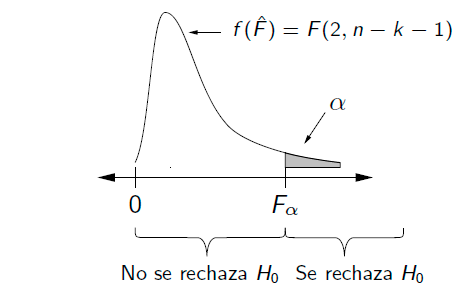
\includegraphics[width=0.7\linewidth]{images/zona.png}
    \end{figure}        
        
        Cuanto más grande sea la diferencia entre los modelos, más extremo será el $F_{\text{empírico}}$
        y más probable que rechacemos la $H_0$.
    \end{itemize}
\end{frame}

\begin{frame}{Distribución F}
    \begin{figure}
        \centering
        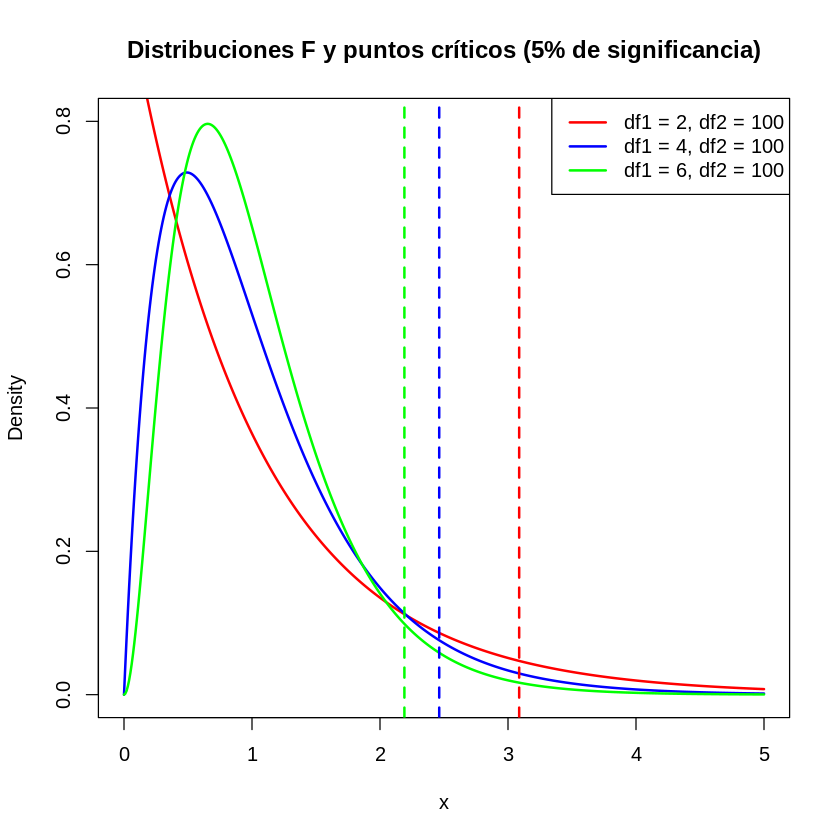
\includegraphics[width=0.7\linewidth]{images/distr_F.png}
    \end{figure}
\end{frame}


\begin{frame}{Ejemplo: rendimiento y salario en el baseball}
    \begin{itemize}
        \item Se tiene el siguiente modelo para los salarios de los jugadores de baseball:
        \[
        \log(\text{salary}) = \beta_0 + \beta_1 \text{years} + \beta_2 \text{gamesyr} + \beta_3 \text{hrunsyr} + \beta_4 \text{rbisyr} + u
        \]
        donde \underline{years} es el número de años en la liga, \underline{gamesyr} el promedio de juegos
        anuales, \underline{hrunsyr} el número de home runs y \underline{rbisyr} el número de corridas
        gracias a su bateo.
        \item Se quiere testear que el rendimiento de los jugadores no influye en sus
        salarios, es decir,
        \[
        H_0 : \beta_3 = \beta_4 = 0 
        \]
        \[
        H_1 : \text{.Al  menos uno es} \ \neq 0
        \]
    \end{itemize}
\end{frame}

\begin{frame}[t, shrink=10]{Ejemplo: rendimiento y salario en el baseball (n=353)}
    \begin{itemize}
        \item \textbf{Step 1:} $H_0: \beta_3 = \beta_4 = 0$, $H_1: \beta_3 \neq 0$ o $\beta_4 \neq 0$
        \item \textbf{Step 2:}
        \begin{enumerate}
            \item \textbf{Modelo no restringido:}
            \[
            \log(\text{salary}) = \beta_0 + \beta_1 \text{years} + \beta_2 \text{gamesyr} + \beta_3 \text{hrunsyr} + \beta_4 \text{rbisyr} + u
            \]
            \textcolor{red}{obtenemos $SSR_{ur}$.}
            \item \textbf{Modelo restringido:}
            \[
            \log(\text{salary}) = \gamma_0 + \gamma_1 \text{years} + \gamma_2 \text{gamesyr} + e
            \]
            \textcolor{red}{obtenemos $SSR_{r}$.}
        \end{enumerate}
        \item \textbf{Step 3:} Calcular $F_{\text{estadístico}} = \frac{(SSR_{r} - SSR_{ur})}{SSR_{ur}} \cdot \frac{353 - 5}{2}$
        \item \textbf{Step 4:} Comparar con el $F$ de la distribución $F(2, 348)$ para 5\% de significatividad.
    \end{itemize}
\end{frame}


\begin{frame}[shrink=10]{Ejemplo: rendimiento y salario en el baseball}
    \begin{itemize}
        \item \textcolor{red}{Resultados modelo no restringido:
        $
        \log(\text{salary}) = \beta_0 + \beta_1 \text{years} + \beta_2 \text{gamesyr} + \beta_3 \text{hrunsyr} + \beta_4 \text{rbisyr} + u
        $}

             \begin{figure}
        \centering
        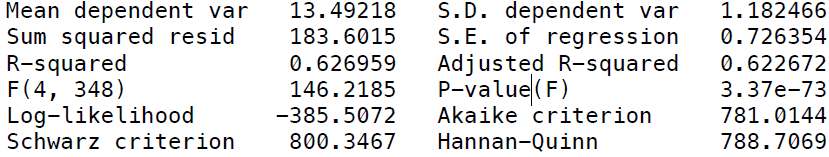
\includegraphics[width=0.8\linewidth]{images/nrsalary.png}
    \end{figure}
        
        \item \textcolor{blue}{Resultados modelo restringido:\\        
        $
        \log(\text{salary}) = \gamma_0 + \gamma_1 \text{years} + \gamma_2 \text{gamesyr} + u
        $}
             \begin{figure}
        \centering
        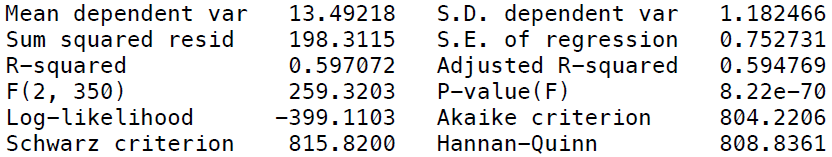
\includegraphics[width=0.8\linewidth]{images/rsal.png}
    \end{figure}    
    \end{itemize}
\end{frame}

\begin{frame}[shrink=10]{Ejemplo: rendimiento y salario en el baseball}
    \begin{itemize}
        \item \textcolor{red}{Resultados modelo no restringido:
        $
        \log(\text{salary}) = \beta_0 + \beta_1 \text{years} + \beta_2 \text{gamesyr} + \beta_3 \text{hrunsyr} + \beta_4 \text{rbisyr} + u
        $}

             \begin{figure}
        \centering
        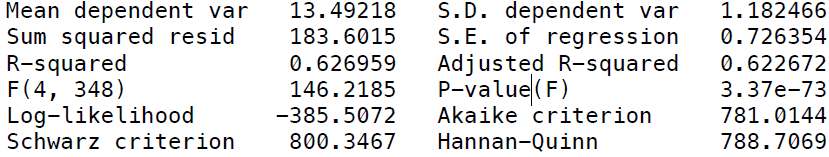
\includegraphics[width=0.8\linewidth]{images/nrsalary.png}
    \end{figure}
        
        \item \textcolor{blue}{Resultados modelo restringido:
        $
        \log(\text{salary}) = \gamma_0 + \gamma_1 \text{years} + \gamma_2 \text{gamesyr} + u
        $}
             \begin{figure}
        \centering
        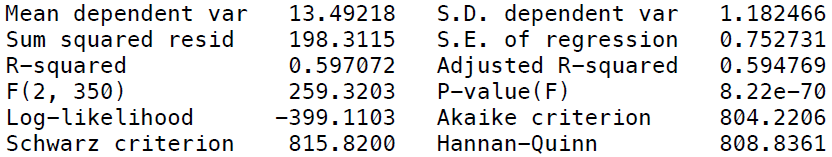
\includegraphics[width=0.8\linewidth]{images/rsal.png}
    \end{figure}
        
        \item Test de hipótesis conjunto para $H_0 : \beta_3 = \beta_4 = 0$
        \[
        F = \frac{(198.31 - 183.60)}{183.60} \cdot \frac{353-4-1}{2} = 13.94
        \]

        \item Comparamos con el punto crítico de $F(2, 348)$  con 5\% de significancia que es 3.02, por lo que rechazamos la hipótesis nula. Es decir, los home runs o las corridas son importantes para explicar el salario.
    \end{itemize}
\end{frame}

\begin{frame}{Ejercicio}
    Use los datos de las tablas anteriores para comprobar que uno también puede
    calcular el $F$-estadístico usando la fórmula con los $R^2$ de los modelos restringidos y
    no restringidos:

   
    \[
    F = \frac{(0.6270 - 0.5971)}{(1 - 0.6270)} \cdot \frac{353 - 4 - 1}{2} = 13.94
    \]

% \begin{figure}
%     \centering
%     
\includegraphics[width=0.8\linewidth]{clase8//images/image.png}
% \end{figure}

    
\end{frame}



\begin{frame}{Ejemplo: rendimiento y salario en el baseball}
             \begin{figure}
        \centering
        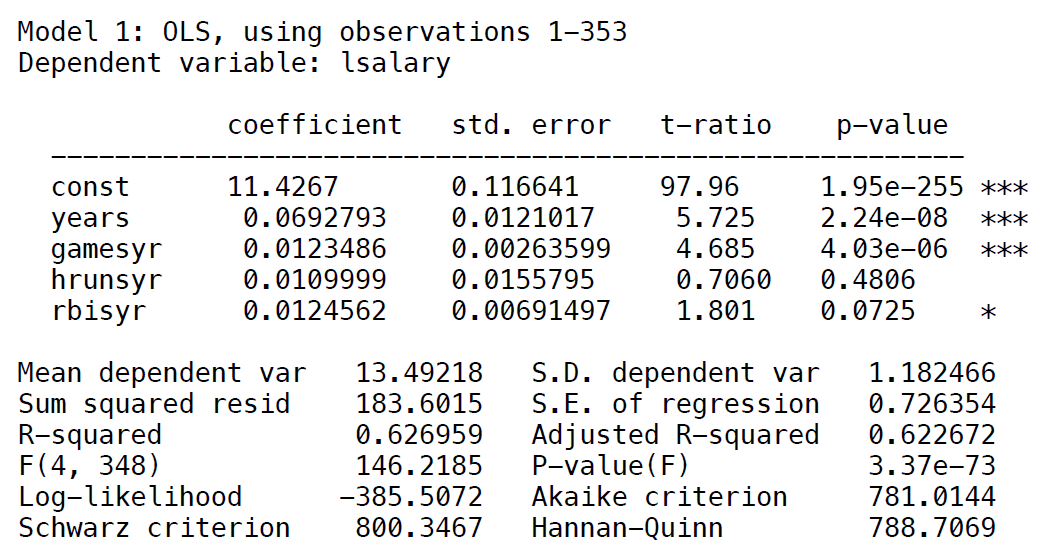
\includegraphics[width=0.8\linewidth]{images/bsbl.png}
    \end{figure}

    \begin{itemize}
    \item Noten que si bien encontramos que los coeficientes conjuntamente son diferentes a 0, los coeficientes para \underline{hrunsyr} y \underline{rbisyr} son positivos, sin embargo, no es posible rechazar la insignificancia individual de cada uno de ellos (con $\alpha = 5\%$).
\end{itemize}
\end{frame}

\begin{frame}[shrink=10]{F-test y el problema de multi-colinealidad}
    \begin{itemize}
        \item Noten que en el ejemplo anterior, no podíamos rechazar que cada coeficiente
        era diferente de 0 por separado.
        \item Sin embargo, el $F$ nos dice que al menos uno de ellos sí lo es. ¿Por qué?
        \item Las variables \textit{hrunsyr} y \textit{rbisyr} están muy correlacionadas y esta
        multicolinealidad dificulta descubrir el efecto parcial de cada variable (dejando
        la otra fija). Esto se refleja en altas varianzas de los estimadores y bajos
        estadísticos $t$ individuales.
        \item Recuerden que si tengo mucha correlación entre dos variables, la varianza de
        sus estimadores aumenta, haciendo más fácil no rechazar la nula.
        \item Sin embargo, el $F$-test al considerarlas juntas, no tiene ese problema y por eso
        es bueno para probar la exclusión de un conjunto de variables.
        \item Por ejemplo, suponga que quieren ver si el desempeño de una empresa afecta
        sueldos de CEOs. Hay muchas medidas para medir desempeño y seguramente
        están correlacionadas (e.g., profits, ventas, etc.). Entonces puede emplearse
        una prueba $F$ para determinar si, como grupo, las variables de desempeño de
        la empresa afectan el sueldo.
    \end{itemize}
\end{frame}

\begin{frame}{Caso particular: Prueba de significancia global}
    \begin{itemize}
        \item Prueba de significación global.
        \item La hipótesis nula es que el modelo entero no explica $y$:
        \[
        H_0 : \beta_1 = \cdots = \beta_k = 0
        \]
        \item En este caso, el modelo restringido es: $y = \beta_0 + u$.
        \item El valor de $R^2_r$ para el modelo restringido es cero. ¿Por qué?
        \item Entonces el estadístico
        \[
        F = \frac{\textcolor{red}{(R^2_{ur} - R^2_{r}})}{(1 - R^2_{ur})} \cdot \frac{n - k - 1}{k} \sim F(k, n - k - 1)
        \]
        \item se reduce a
        \[
        F = \frac{R^2}{1 - R^2} \cdot \frac{n - k - 1}{k}
        \]
        \item donde $R^2$ es el valor obtenido en el modelo sin restringir.
        
    \end{itemize}
\end{frame}

% \begin{frame}{Tabla ANOVA}
%     \begin{tabular}{|c|c|c|c|}
%         \hline
%         & Suma de cuadrados & Grados de libertad & Suma promedio \\ 
%         &                   &                    & de cuadrados \\
%         \hline
%         Regresión & SSE & $k$ & $SSE/k$ \\

%         Residuos & SSR & $n - k - 1$ & $SSR/n - k - 1$ \\
%         \hline
%         Total & SST & $n - 1$ & $SST/n - 1$ \\
%         \hline
%     \end{tabular}
    
%     \begin{itemize}
%          \item Ejemplo:

%              \begin{figure}
%         \centering
%         
\includegraphics[width=0.7\linewidth]{clase8/images/ANOVA.png}
%     \end{figure}
    
%         \item Se rechaza la hipótesis nula
%         \[
%         F = \frac{0.6270}{(1 - 0.6270)} \cdot \frac{353 - 4 - 1}{4} = 146.22
%         \]
%     \end{itemize}
% \end{frame}

% \begin{frame}{Gráfico Distribución F en R}
%     \begin{figure}
%         \centering
%         
\includegraphics[width=0.89\linewidth]{clase8/images/image_prog.png}
%     \end{figure}
% \end{frame}




\end{document}
